\chapter{Solving the Bogoliubov-de Gennes Hamiltonian for a triangular lattice}
\section{Finite lattice real space}
The Bogoliubov-de Gennes (BdG) Hamiltonian is commonly used for describing quasiparticle excitations in superconductors. In this work we will solve the BdG equation for a topological  superconductor on an equilateral triangle of finite lattice sites. An equilateral triangle is chosen because it is topologically equivalent to a T-junction which is commonly used for illustrating braiding operations of Majorana fermions in 1D topological superconductors. 

We solve the system numerically for finite lattice sites. Begin by starting with the tight-binding Hamiltonian for a $\vec{p}$-wave superconductor on a triangular lattice
\begin{equation}
\mathcal{H} = \sum\limits_{i} (6t-\mu)c^{\dagger}_{i}c_{i} + \sum\limits_{<i,j>} \left(-tc^{\dagger}_{i}c_{j} + \Delta e^{i\phi_{ij}}c^{\dagger}_{i}c^{\dagger}_{j} + h.c.\right).
\end{equation}

To get to the BdG Hamiltonian we need to use the anticommutation relation for fermions
\begin{align}
\{c_i,c_j\} &= \{c_i^\dagger,c_j^\dagger\} = 0 \\
\{c_i^\dagger,c_j\} &= c_i^\dagger c_j + c_j c_i^\dagger = \delta_{ij},
\end{align}

Which allows us to write the operators as
\begin{align}
c_i^\dagger c_j &= \frac{1}{2}(c_i^\dagger c_j - c_j c_i^\dagger + \delta_{ij}) \\
c_i c_j &= \frac{1}{2}(c_i c_j - c_j c_i ).
\end{align}

Using the Nambu spinor in lattice space and momentum space
\begin{align}
  \Psi &\equiv (c_1,\cdots,c_N,c_1^\dagger,\cdots,c_N^\dagger)^T \\
  \Psi &\equiv (c_k, c_{-k}^\dagger)^T
\end{align}

We can rewrite the tight-binding Hamiltonian as
\begin{equation}
\mathcal{H} = \frac{1}{2}\Psi^{\dagger}H_{BdG}\Psi.
\label{eqn=CompactHamiltonian}
\end{equation}

The HdG Hamiltonian is then solved numerically using a python script (REFERENCE SRC HERE). 
\section{Infinite lattice momentum space}
We then solve our problem in momentum space for an infinite triangular lattice. Starting back at the tight-binding Hamiltonian we take the fourier transform of the creation and annihilation operators where
\begin{equation}
  c_i = \frac{1}{\sqrt{N}} \sum\limits_{\vec{k}} c_k e^{-i\vec{k}\cdot\vec{r_i}}.
\end{equation}

Following the sames steps as mentioned before we arrive at the same compact form as Eqn. \ref{eqn=CompactHamiltonian} where the BdG Hamiltonian is simply a $2\times2$ matrix 

\[
H_{BdG}=
  \begin{bmatrix}
   t(\vec{k}) & \Delta(\vec{k})\\
   \Delta^{\star}(\vec{k}) & -t(\vec{k})
  \end{bmatrix}.
\]

The functions of the BdG matrix are 
\begin{align}
t(\vec{k}) &= -2t\left[\cos(ak_x) + \cos\left(\frac{ak_x}{2}+\frac{\sqrt{3}ak_y}{2}\right) + \cos\left(\frac{ak_x}{2}-\frac{\sqrt{3}ak_y}{2}\right)\right] - (\mu - 6t) \\
\Delta(\vec{k}) &= 2\Delta i \left[\sin(ak_x)-e^{\frac{4\pi i}{3}}\sin\left(\frac{ak_x}{2}+\frac{\sqrt{3}ak_y}{2}\right) + e^{\frac{5\pi i}{3}}\sin\left(\frac{ak_x}{2}-\frac{\sqrt{3}ak_y}{2}\right)  \right]
\end{align}

The determinant of this matrix is easily solved to give the energy eigenvalues as $E = \pm\sqrt{t(\vec{k})^2 + \|\Delta(\vec{k})\|^2 }$.

\section{Results}
NEED TO FINISH THIS SECTION (FIXED THE FIGURE LABELS OF THE FIGURES AND REFERENCES)
The numerical approach to solving the finite triangle has some hangups. The BdG Hamiltonian is of the size $ 2N \times 2N $ and eigenvalue solvers run on the order of $\mathcal{O}(n^3)$. This severly dampens the ability to simulate a physically realizable triangular lattice. Aside from that we can still get meaningful physical phenomena from using a small triangular lattice. Let us first look at the energy spectra of both the finite lattice in real space and infinite lattice in momentum space. The momentum energy spectra seen in Fig. \ref{fig-momspectra} shows an apparent energy band gap of $\Delta\epsilon = \pm2(t)$ while the real space energy spectra in Fig \ref{fig-enespectra} shows energy values lying within the energy band gap.

\begin{figure}
%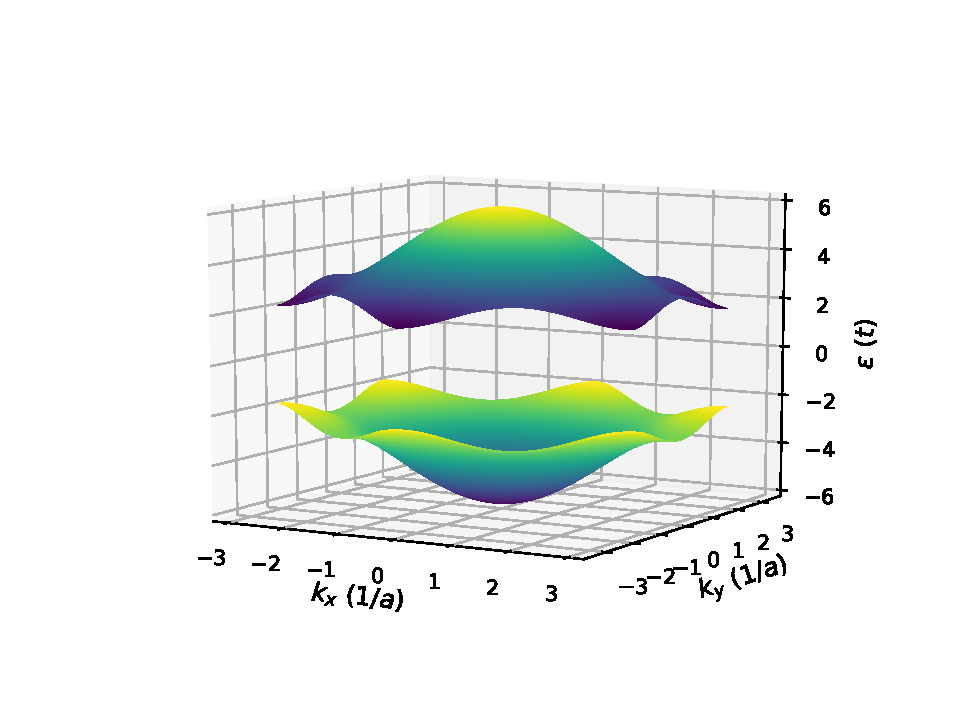
\includegraphics[scale=.5]{fig-energy-band-gap-momentum-space.pdf}
\caption{}
\label{fig-momspectra}
\end{figure}

\begin{figure}
%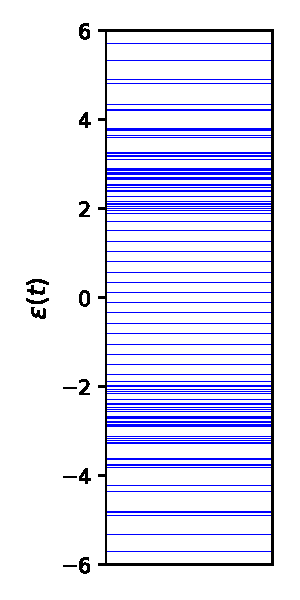
\includegraphics[scale=.5]{fig-energy-spectra.pdf}
\caption{}
\label{fig-enespectra}
\end{figure}

\begin{figure}
%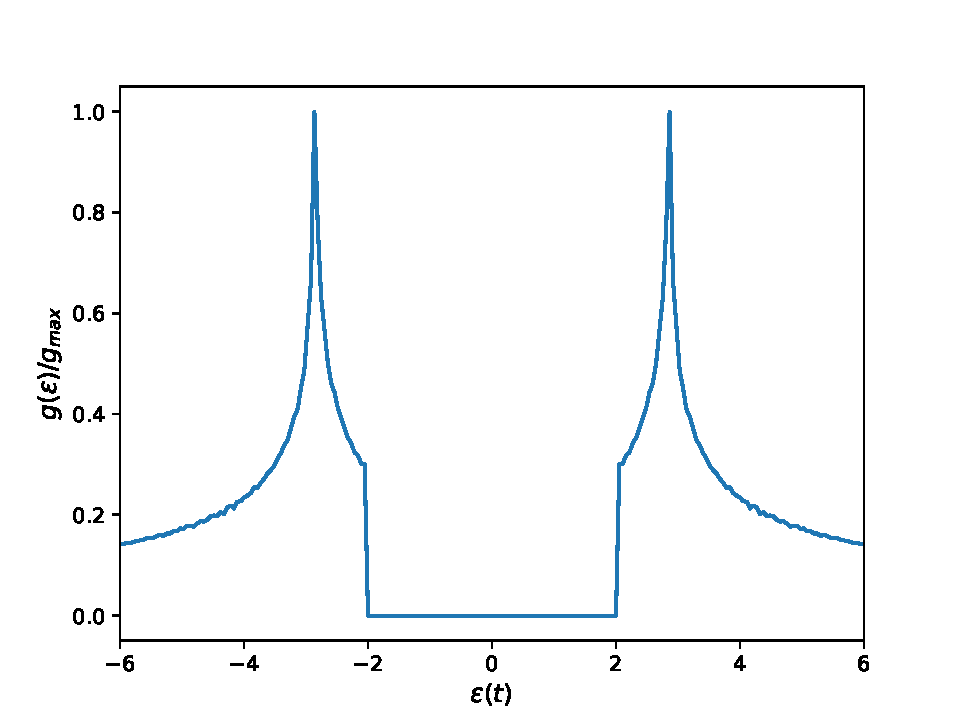
\includegraphics[scale=.5]{fig-dos-momentum.pdf}
\caption{}
\label{fig-dosmom}
\end{figure}

\begin{figure}
%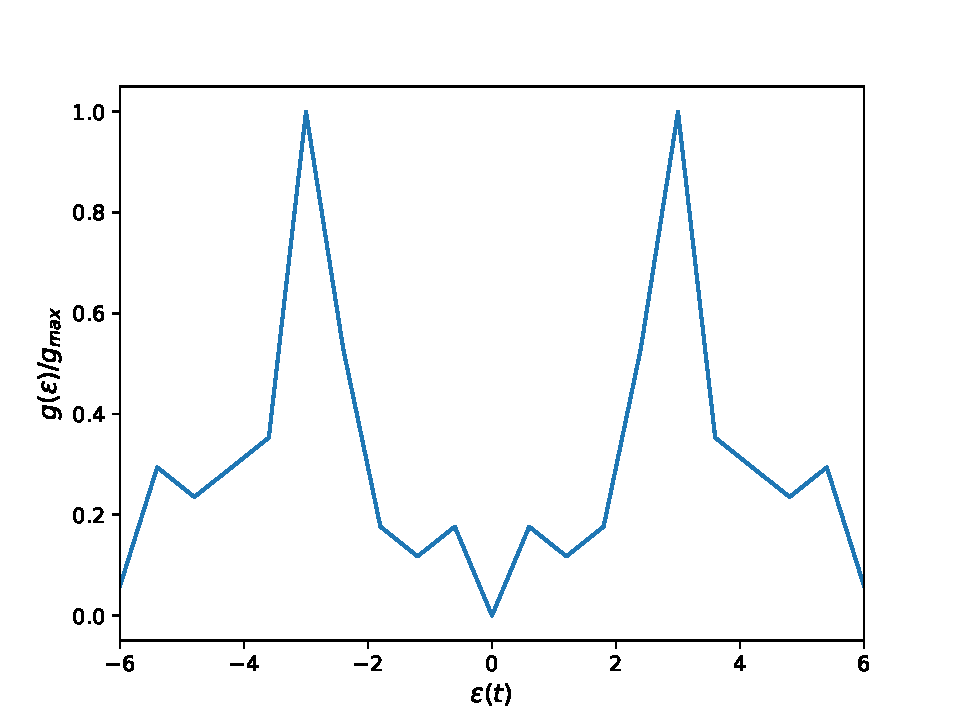
\includegraphics[scale=.5]{fig-dos-real-space.pdf}
\caption{}
\label{fig-dosspace}
\end{figure}


